\documentclass[a4paper, 12pt]{article}%тип документа

%отступы
\usepackage[left=0.6cm,right=1cm,top=2cm,bottom=3cm,bindingoffset=0cm]{geometry}
\setlength{\parindent}{5ex}

%Русский язык
\usepackage[T2A]{fontenc} %кодировка
\usepackage[utf8]{inputenc} %кодировка исходного кода
\usepackage[english,russian]{babel} %локализация и переносы

%Вставка картинок
\usepackage{graphicx}
\graphicspath{{pictures/}}
\DeclareGraphicsExtensions{.pdf,.png,.jpg}

%Графики
\usepackage{pgfplots}
\pgfplotsset{compat=1.9}

%Математика
\usepackage{amsmath, amsfonts, amssymb, amsthm, mathtools}

%Таблицы
\usepackage{longtable} 
\usepackage{float}

%Римские цифры
\newcommand{\RomanNumeralCaps}[1]{\uppercase\expandafter{\romannumeral#1}}

\usepackage{multirow}


\begin{document}
\begin{titlepage}
\begin{center}
\textsc{Федеральное государственное автономное образовательное учреждение высшего образования«Московский физико-технический институт (национальный исследовательский университет)»\\[5mm]
}

\vfill

\textbf{Отчёт по лабораторной работы 4.2.1 \\[3mm]
КОЛЬЦА НЬЮТОНА
\\[50mm]
}

\end{center}

\hfill
\begin{minipage}{.5\textwidth}
Выполнил студент:\\[2mm]
Сериков Алексей Романович\\[2mm]
группа: Б03-103\\[5mm]

\end{minipage}
\vfill
\begin{center}
Москва, 2023 г.
\end{center}

\end{titlepage}

\newpage
\textbf{Аннотация}\\


\textbf{Цель работы: }\\

Познакомиться с явлением интерференции в тонких плёнках (полосы равной толщины) на примере колец Ньютона и с методикой интерференционных измерений кривизны стеклянной поверхности.

	\textbf{В работе используются: }\\
	
Измерительный микроскоп с опак-иллюминатором, плоско-выпуклая линза; пластинка из чёрного стекла, ртутная лампа типа ДРШ, щель, линзы, призма прямого зрения, объектная шкала.\\



\textbf{Теория:}


\begin{figure}[H]
	\begin{center}
		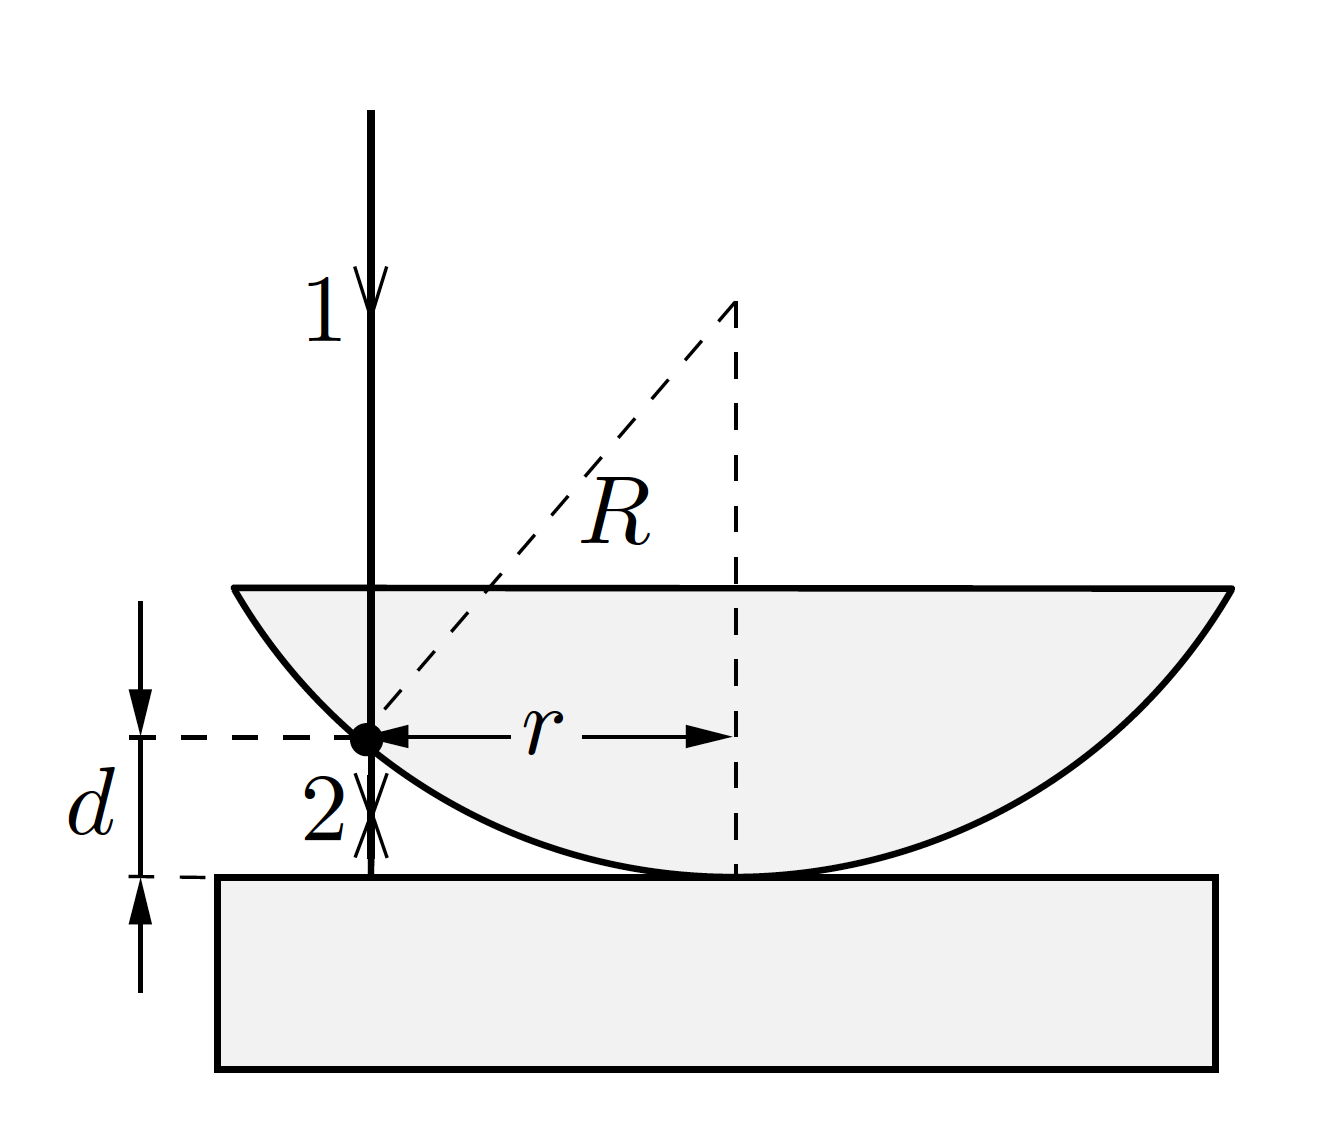
\includegraphics[width=0.5\linewidth]{Lens.png}
		\caption{Линза}
	\end{center}
\end{figure}



Этот классический опыт используется для определения радиуса кривизны сферических поверхностей линз. В этом опыте наблюдается интерференция волн, отражённых от границ тонкой воздушной прослойки, образованной сферической поверхностью линзы и плоской стеклянной пластиной. При нормальном падении света (рис. 1) интерференционные полосы локализованы на сферической поверхности и являются полосами равной толщины.

Геометрическая разность хода между интерферирующими лучами равна удвоенной толщине воздушного зазора $ 2d $ в данном месте. Для точки на сферической поверхности, находящейся на расстоянии $ r $ от оси системы, имеем $ r^2 = R^2 - (R - d)^2 = 2Rd - d^2 $, где $ R $ --- радиус кривизны сферической поверхности (рис. 1).

При $ R \gg d $ получим$  d = r^2/2R $. С учётом изменения фазы на $ \pi $ при отражении волны от оптически более плотной среды (на границе воздух-стекло) получим \textbf{оптическую разность хода интерферирующих лучей}:

\begin{equation}\label{r_m}
	\Delta = \dfrac{\lambda}{2} + 2d = \dfrac{r^2}{2R} + \dfrac{\lambda}{2}
\end{equation}

Из условия интерференционного минимума $ \Delta = \dfrac{(2m +1)\lambda}{2}, \; m =0, 1, 2.. $ получим радиусы темных колец $ r_m $, а из аналогичного условия максимума $ \Delta = m \lambda $ радиусы светлых $ r_m' $ :

\begin{equation}\label{r_m'}
	r_m = \sqrt{m \lambda R}, \qquad 	r_m' = \sqrt{\dfrac{(2m-1)m \lambda R}{2}}
\end{equation}

\textbf{Экспериментальная установка:}

Схема экспериментальной установки приведена на рис. 2. Опыт выполняется с помощью измерительного микроскопа.
На столик микроскопа помещается держатель с полированной пластинкой из
чёрного стекла. На пластинке лежит исследуемая линза.

\begin{figure}[H]
	\begin{center}
		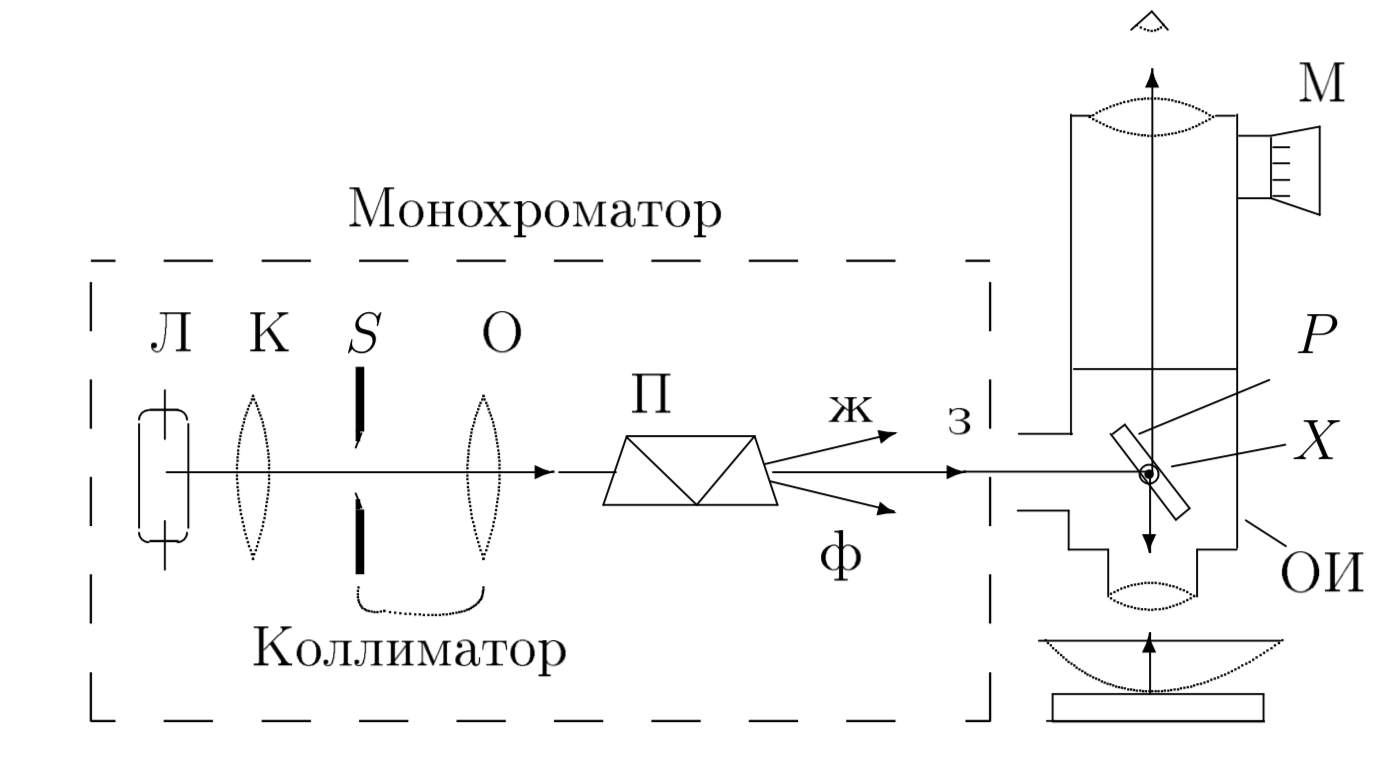
\includegraphics[width=0.6\linewidth]{Lab.png}
		\caption{Экспериментальная установка}
	\end{center}
\end{figure}

Источником света служит ртутная лампа, находящаяся в защитном кожухе. Для получения монохроматического света применяется призменный монохроматор, состоящий из конденсора $ К $, коллиматора (щель $ S $ и объектив $ О $) и призмы прямого зрения $ П $. Эти устройства с помощью рейтеров располагаются на оптической скамье. Свет от монохроматора попадает на расположенный между объективом и окуляром микроскопа опак-иллюминатор (ОИ)  специальное устройство, служащее для освещения объекта при работе в отражённом свете. Внутри опак-иллюминатора находится полупрозрачная стеклянная пластинка P, наклоненная под углом $ 45^\circ $ к оптической оси микроскопа. Свет частично отражается от этой пластинки, проходит через объектив микроскопа и попадает на исследуемый объект. Пластинка может поворачиваться вокруг горизонтальной оси $ X $, опак-иллюминатор вокруг вертикальной оси.

Столик микроскопа может перемещаться в двух взаимно перпендикулярных направлениях помощью винтов препаратоводителя. Отсчетный крест окулярной шкалы перемещается перпендикулярно оптической оси с помощью микрометрического винта $ М $.

Оптическая схема монохроматора позволяет получить в плоскости входного окна опак-иллюминатора достаточно хорошо разделённые линии спектра ртутной лампы. Изображение щели $ S $ фокусируется на поверхность линзы объективом микроскопа, т.е. точка источника и точка наблюдения спектра совпадают.Интерференционная картина не зависит от показателя преломления линзы и определяется величиной зазора между линзой и пластинкой (кольца равной толщины).

Сначала микроскоп настраивается на кольца Ньютона в белом свете (свете ртутной лампы), затем при помощи монохроматора выделить из спектра яркую зелёную линию и провести измерения диаметров колец в монохроматическом свете. 

\newpage

	\textbf{Ход работы и обработка результатов.}\\
	

	После настройки микроскопа проведем измерения диаметров колец Ньютона. Измерения будем проводить в безразмерных единицах окулярной шкалы, переведённых затем в реальную величину с помощью калиброванной объектной шкалы. 


C помощью призмы выделим зеленый свет из спектра лампы ($ \lambda_{green} = 546 $ нм).

Будем последовательно измерять координаты экстремумов $ l $. Результаты занесем в Таблицу 1, зная, что 100 дел соответствует 0.1мм



\begin{longtable}{|c|c|c|c|c|c|}
			\hline
			m      & $l_{dark}$, мкм & $l_{light}$, мкм & $r_{dark}^2$, нм & $r_{light}^2$, нм 					 \\ \hline
			0 	   & 0             & 0              & 0                       & 0 						     \\ \hline
			1      & 81            & 59            	& 6.56                    & 3.48 				     \\ \hline
			2      & 120           & 103            & 14.4                    & 10.60 					 \\ \hline
			3      & 145           & 133            & 21.02                   & 17.69                    \\ \hline
			4      & 168           & 158            & 28.22                   & 24.96                     \\ \hline
			5      & 187           & 182            & 24.96                   & 33.12                    \\ \hline
			6      & 205           & 200            & 42.02                   & 40.00                   \\ \hline
			7      & 222           & 217            & 49.28                   & 47.09                       \\ \hline
			8      & 239           & 235            & 57.12                   & 55.22                     \\ \hline
			9      & 255           & 252           	& 65.02                   & 63.50                      \\ \hline
			10     & 268    	   & 264         	& 71.82                   & 69.69                      \\ \hline
			11     & 282           & 277           	& 79.52                   & 76.72                   \\ \hline
			12     & 293           & 290           	& 85.85                   & 84.10                     \\ \hline
\caption{Таблица с данными координат и радиусов тёмных и светлых колец Ньютона.}
\end{longtable}

Построим график зависимости $r^2$ от m для светлых и тёмных колец:

\begin{figure}[H]
	\begin{center}
		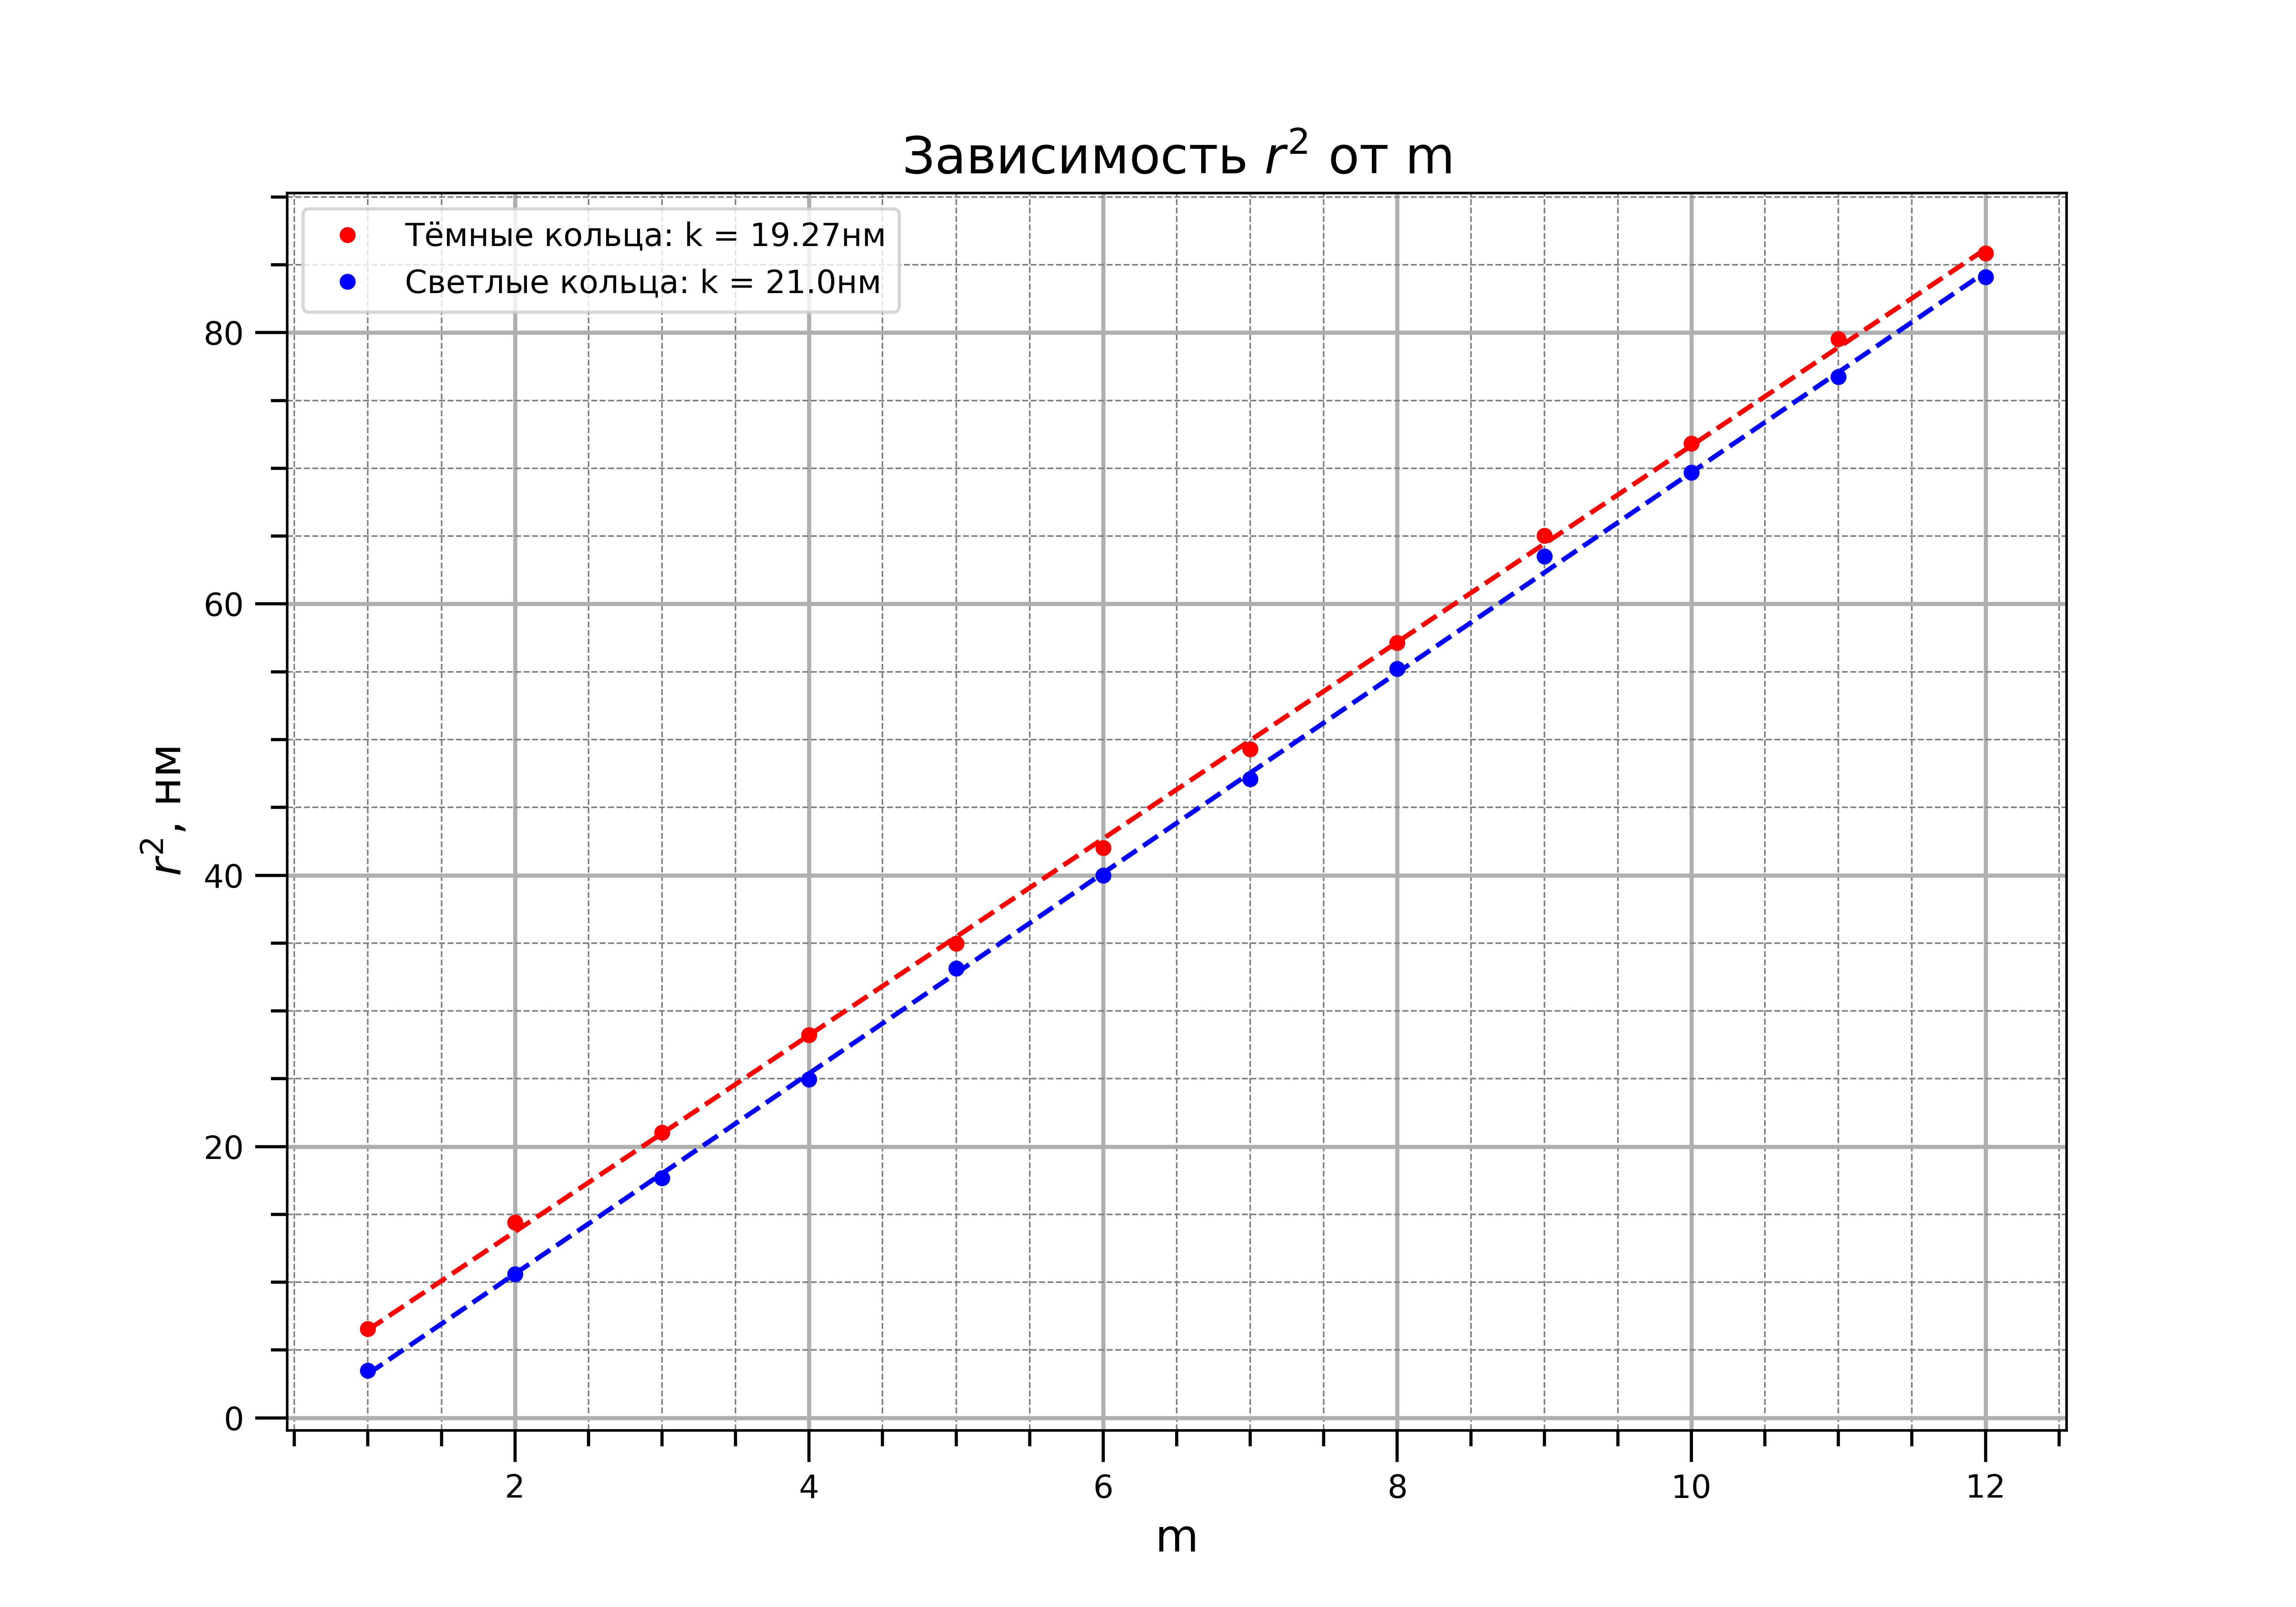
\includegraphics[width=0.6\linewidth]{r(m).png}
		\caption{Экспериментальная установка}
	\end{center}
\end{figure}


Наблюдая биения, определили, что на промежутке между двумя центрами соседних четких участков укладывается $\Delta m$ = 19 колец. Тогда получим:

\begin{equation}
	\Delta\lambda = \frac{\lambda_{green}}{\Delta m} = 28.7 \text{нм}.
\end{equation} 

По формуле (2) и коэффициенту наклону $k$ определим радиус кривизны $R$:

$R = (3.6 \pm 0.1$)см.

	\textbf{Обсуждение результатов и выводы: }\\
В работе мы, измерив диаметры колец Ньютона, определили радиус кривизны линзы, исследовали картину биений и рассчитали
разность длин волн между жёлтой и зелёной спектральными линиями
ртути.


\end{document}
